\chapter{Discussion}

\epigraph{\textit{These thoughts are constructive criticisms. Pyramidical. I try to suppress these thoughts, but they leak out...}}{George Saden -- \textit{Zardoz}}

\vspace{1cm}

\par\noindent In Chapters \ref{ch:IGR} and \ref{ch:BPbig}, I discuss new ways of classifying variability in the unusual LMXBs IGR J17091 and the Bursting Pulsar.  I use the new classification frameworks I have created to compare these objects with the similar LMXBs GRS 1915 and the Rapid Burster respectively.  While I find a number of similarities between these objects, I also highlight a number of differences.  For example, I find that the spectral evolution during variability in IGR J17091 is very different to in GRS 1915, and the bursts in the Bursting Pulsar evolve in a very different way to those seen from the Rapid Burster.
\par A common theme throughout work presented in this thesis is that the variability in these unusual objects is even more complex than had previously been thought.  Application of Occam's razor \citep{Occam} suggests that the similar variability from these objects is generated by similar physics, but I have found that it is difficult to unify the diverse behaviours of these unusual systems.  I also compare the four objects that I focus on with other unusual XRBs such as Terzan 5 X-2 and, in Chapter \ref{ch:BPletter}, TMSPs.  In this chapter I discuss the relationships between these seemingly disparate objects, and how my findings fit in to the more general picture of accretion in these extreme and bizarre systems.

\section{General Observations}

\label{sec:disccomp}

\subsection{Variability Evolution throughout an Ouburst}

\par One feature common to at least 3\footnote{As GRS 1915 has been in outburst since its discovery, it is unknown how its variability classes vary as a function of where it is in an outburst.} of the unusual LMXBs discussed in this thesis is that variability changes in a predictable way over the course of an outburst.  This effect is most apparent in the results I present in Chapter \ref{ch:BPbig}, where I discuss an evolution of bursting which is observed in both the 1996 and 1997 outbursts of the source:
\begin{itemize}
\item Normal Bursts and Minibursts begin to occur shortly after the peak of the outburst.
\item Bursting shuts off entirely when the persistent flux of the source decreases below $\sim0.1$\,Crab.
\item The persistent flux of the system increases in a rebrightening event, at which point Mesobursts begin to occur.
\item Mesobursts evolve into Structured Bursting.
\end{itemize}
\par A predictable evolution of bursting throughout an outburst has also been identified in the Rapid Burster (e.g. \citealp{Bagnoli_PopStudy}).  In this system, bursts near the start of each outburst are Eddington-Limited and persist for $\sim100$s of seconds (see e.g. the upper panel of Figure \ref{fig:bagnoli_lcs}).  As the outburst persists, these bursts become shorter, fainter and more sharply peaked (see e.g. the lower panel of Figure \ref{fig:bagnoli_lcs}).  This evolution is qualitatively very different from the evolution of bursting seen in the Bursting Pulsar.  However, the fact that bursting in both objects changes in a predictable way throughout each outbursts shows that bursting in both objects is dependent on the accretion rate in the system and on the state of its accretion disk.
\par There is also some evidence of an evolution of bursting in IGR J17091.  In Figure \ref{fig:WhereCls} we show a number of lightcurves of the 2011 outburst of IGR J17091, highlighting when in the outburst each of our 9 variability classes was observed.  Although the evolution between classes is much less `neat' than in the Bursting Pulsar, it is easy to identify a number of patterns in the data, such as:
\begin{itemize}
\item Class I only occurs near the start of the outburst, within 25 days of the onset of variability.
\item Class II only occurs during two dips in the persistent flux to a level of $\sim20$\,mCrab.
\item Class VII only occurs while the persistent flux of IGR J17091 is in a narrow band centred on $\sim70$\,mCrab.
\end{itemize}
It is unclear whether a similar evolution occurs during the 2016 outburst of IGR J17091, as a variability population study for this outburst has not yet been performed.  However these results from the 2011 outburst suggest that variability in IGR J17091 also depends strongly on the accretion rate and the state of the disk, as it is in the Rapid Burster and the Bursting Pulsar.

\subsection{Criteria for Exotic Variability}

\par As we show in Figure \ref{fig:IGR2016}, the 2016 outburst of IGR J17091 showed a number of the classes of variability which it showed in 2011 (e.g. \citealp{Reynolds_2016HB}).  The bursting in 1996 and 1997 outbursts of the Bursting Pulsar evolved in nearly exactly the same way (see e.g. Section \ref{sec:bburstevo}), and the Rapid Burster goes into outburst regularly every $\sim$100--200 days and always displays Type II bursts.  These observations strongly suggest that the ability to produce Type II bursting or GRS 1915-like variability is a property of the system rather than of an individual outburst.  In these systems some set of parameters, which persist between outbursts, are just right to allow these exotic types of variability to occur.

\begin{figure}
  \centering
  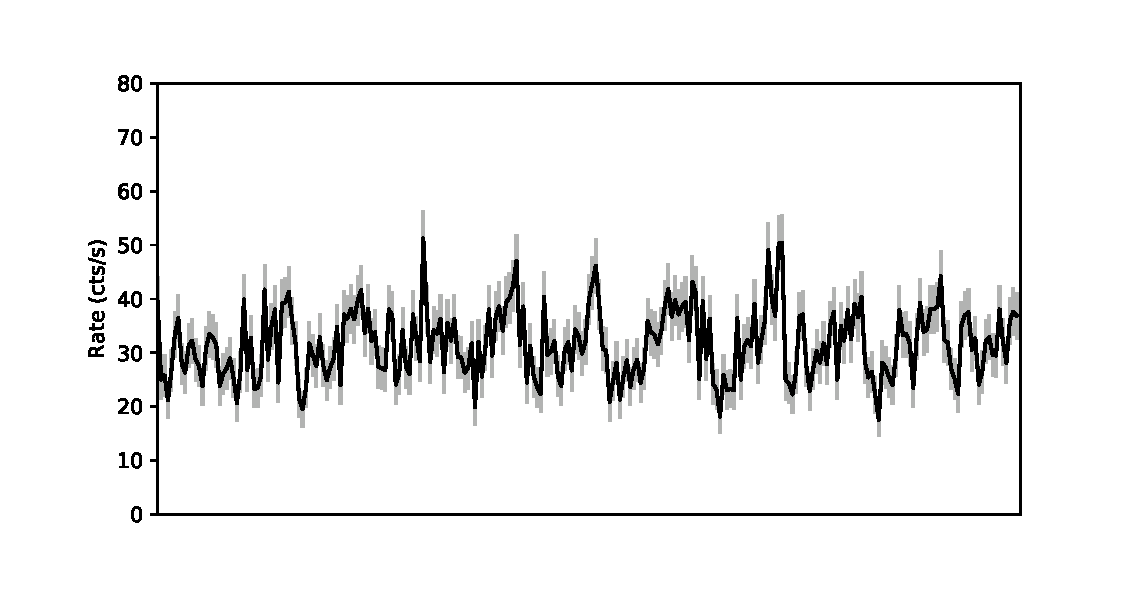
\includegraphics[width=.9\linewidth, trim= 10mm 8mm 10mm 10mm,clip]{images/2016_III.eps}
  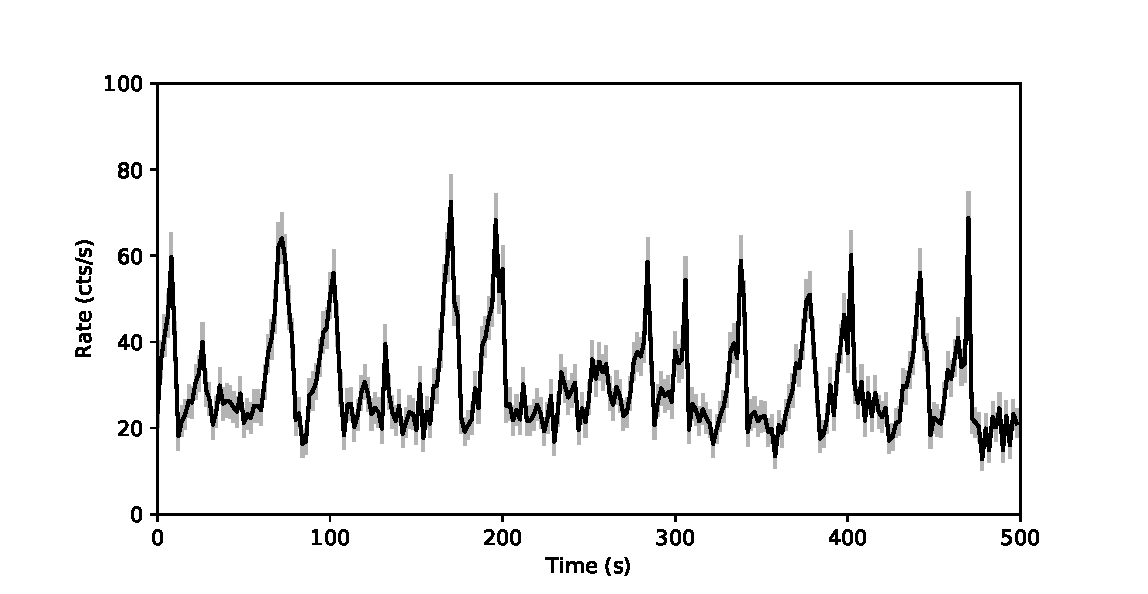
\includegraphics[width=.9\linewidth, trim= 10mm 0mm 10mm 10mm,clip]{images/2016_V.eps}
  \caption[\textit{Swift}/XRT lightcurves of IGR J17091-3624 during its 2016 outburst, showing two of the variability classes we identify in Chapter \ref{ch:IGR}.]{0.3--10\,keV \textit{Swift}/XRT lightcurves of IGR J17091-3624 during its 2016 outburst.  In the top panel, the source is undergoing Class III variability, while in the bottom panel it is undergoing Class V variability.}
  \label{fig:IGR2016}
\end{figure}

\par Compact objects, and by extension LMXBs, are relatively simple systems which can be well-defined with only a few parameters.  The compact object in such a system can be described using only the following parameters:

\begin{itemize}
\item The type of object (neutron star or black hole).
\item Mass.
\item Spin and rate of change of spin.
\item Magnetic Field Strength.
\end{itemize}

Where the last parameter only applies if the object is a neutron star.  In addition to these, one only has to describe the companion star (mass, mass loss rate, spectral type etc.), the parameters of the system orbit (eccentricity, semi-major axis and misalignment from the spin axes of both stars) and the mass transfer rate to fully describe the system.  Due to this relative simplicity, there are not many candidates for parameters which govern the existence of exotic variability.  GRS 1915+105 contains the highest mass black hole known in an LMXB\footnote{At least one HMXB, Cyg X-1, is believed to contain a black hole with higher mass \citep{Orosz_CygX1}.} ($12.4\pm2.0$\,M$_\odot$, \citealp{Reid_Parallax}), although many other LMXBs are believed to contain black holes with comparable masses (e.g. V404 Cyg, \citealp{Shahbaz_V404}).  The black hole in GRS 1915 also has a very high spin, with a spin parameter of $0.98\pm0.01$ \citep{Miller_GRSspin}, but a number of other XRBs are also believed to harbour near-maximal spin black holes (see e.g. \citealp{Fragos_spin}).  In Chapter \ref{ch:BPletter} we consider a `hiccup'-like accretion behaviour as a possible mechanism behind variability in the Bursting Pulsar; this mechanism relies on specific ranges for the values of spin and magnetic field strength, but cannot be used to explain any of the variability seen in black hole systems.
\par Lense-Thirring precession in the disk, caused by the misalignment of the orbital and spin axes of the compact object, has been used to explain some of the variability seen in LMXBs (e.g. \citealp{Stella_LT}).  However, the timescale of the variability this generates is no slower than $\sim10$\,Hz \citep{Ingram_Solid} too fast to be linked with the $\lesssim0.1$\,Hz variability seen from GRS 1915.  Instead the other parameters on the list, or a combination thereof, must be the determining factors in whether or not an object can display exotic variability.
\par While I find that Eddington-limited accretion is not necessary for either GRS 1915-like variability or Type II bursting, all of the objects considered in this thesis have relatively high accretion rates during the peak of their outbursts: the Rapid Burster, which is the least luminous of the four systems, accretes at $\sim20$\% of its Eddington rate at peak.  While a high accretion rate is obviously not sufficient for GRS 1915-like variability or Type II bursting to occur, as many systems with high accretion rates do not display either behaviour, this result suggests that a high accretion rate may be a necessary criterion.
\par GRS 1915 has a very long orbital period of $\sim30$ days \citep{Neil_GRSPeriod}, and this is believed to result in GRS 1915 having the largest accretion disk of all X-ray binaries.  This likely explains how GRS 1915 has been in outburst for such a long period of time ($\gtrsim20$ years, compared to the $\lesssim2$\,year outburst seen in most LMXBs).  The orbital periods of IGR J17091 and the Rapid Burster are unknown, but the Bursting Pulsar also has a relatively long orbital period of 11.8 days (e.g. \citealp{Finger_BP}), suggesting that a large disk may also be a factor in the generation of exotic variability.
\par \citet{Sadowski_MagField} calculate the minimum magnetic field strength which, when threaded through a radiation-dominated disk undergoing the instability described by \citet{Shakura_Instab}, would be able to stabilise the disk.  Assuming that such a field in an LMXB is provided by the companion star, they find that this minimum value in an LMXB depends mostly on the luminosity of the system and the mass of the compact object.  They estimate the value of the minimum stabilising field strength in a number of black hole X-ray binaries, and find that the field required to stabilise GRS 1915 is $\sim5.7\times10^{11}$\,G\,cm$^{-2}$; this is over twice as large as the second highest value they find for an LMXB (XTE J1550-564).  This high value is due to the large black hole mass in GRS 1915, and the fact that this black hole accretes at a near-Eddington rate and, thus, a high luminosity.  In this picture, therefore, GRS 1915-like variability may simply be a manifestation of the \citet{Shakura_Instab} instability which is suppressed in most LMXBs.  One could test the viability of this scenario by calculating the minimum stabilising field for IGR J17091.  Unfortunately at time of writing no companion star to IGR J17091 has been found, and the mass and distance (and hence luminosity) of the system remain unknown.
\par It is worth noting that this scenario suggested by \citet{Sadowski_MagField} is unable to account for Type II bursts as, in these systems, the neutron star is able to provide more than enough magnetic flux to stabilise the inner disk.  In this case, Type II bursts would have to be explained by some entirely separate physical mechanism, as would the apparent GRS 1915-like variability features in the Rapid Burster reported by \citet{Bagnoli_RB}.

\subsection{Evidence of System Memory}

\par Another notable observation from these objects is that variability in GRS 1915 and IGR J17091 falls into a discrete set of variability classes.  In both objects, a variability class could be observed on one day, not be observed for weeks and then reappear in a form almost identical to the previous sighting.  Somehow these systems `know' which variability classes they are allowed to display.  In Figure \ref{fig:IGR2016} I show evidence that two of the variability classes I identified in the 2011 outburst of IGR J17091 occurred again in 2016.  This suggests that GRS 1915-like systems are somehow able to `remember' which variability class they can occupy, and that this information between outbursts.  This in turn means that, in addition to determining whether or not GRS 1915-like variability can occur, the simple parameters that define a black hole LMXB also determine \textit{which} classes of GRS 1915-variability can occur.
\par In Section, I report that two of the classes of variability I find in IGR J17091 (Classes VII and VIII) are unlike anything which has ever been seen in GRS 1915 (see also Table \ref{tab:class_assign}).  This leads to one of three possibilities:
\begin{itemize}
\item Class VII and VIII like variability has occurred in GRS 1915 since its discovering, but coincidentally we have never observed it.  As GRS 1915 has been observed extensively during its ongoing $\gtrsim20$ year-long outburst, this is unlikely to be true.
\item Class VII and VIII variability preferentially occurs during a specific period in the evolution of an outburst, and GRS 1915 is not currently in this period.
\item Some set of system parameters in IGR J17091 are different from in GRS 1915 in such a way that different classes of variability are permitted.
\end{itemize}
\par The final possibility is of great interest.  Future observations of IGR J17091 will aim to better constrain the parameters that define the system; if these parameters are then compared to the already well-constrained parameters of GRS 1915, then we may be able to learn exactly why Class VII and VIII variability is permitted in one object but not the other.  This in turn may shed further light on physics behind GRS 1915-like variability in general.
\par There is also evidence of some degree of system memory in the Type II bursting systems.  The near-identical evolutions of the 1996 and 1997 outbursts of the Bursting Pulsar indicate that the factors governing outburst evolution also persist between outbursts in this object.
\par The Normal Bursts and Minibursts, which I describe in Sections \ref{sec:Normal_Bursts} and \ref{sec:Minibursts} respectively, also provide evidence of system memory in the Bursting Pulsar.  In Section \ref{sec:Mini_Norm} I discuss the possibility that Minibursts and Normal Bursts are manifestations of the same physical limit cycle.  Both types of burst display a number of similar features, notably including an exponential-shaped dip in count rate after each burst, and they occur interchangeably during the same periods of time in both the 1996 and 1997 outbursts of the source.  Minibursts and Normal Bursts are separated based on their amplitudes.  However, as I show in Figure \ref{fig:minidips}, the amplitudes of both features do not form a single continuous distribution, but rather fall into two well-separated populations.  In both the 1996 and 1997 Outbursts of the Rapid Burster, there are no Normal or Minibursts with fluences between $\sim10^4$ and $\sim10^5$ 2--60\,keV PCA counts.  Due to the large number of Minibursts and Normal Bursts observed in my study, it is highly likely that this gap is real; if we assume that Normal Bursts and Minibursts are the same phenomenon, then there must be some physical reason for this gap which persists between outbursts.  Observations of future outbursts of the Bursting Pulsar will allow us to see whether this fluence gap always spans the same range, or whether this gap drifts during the longer-term evolution of the system.

\section{IGR J17091 vs. the Bursting Pulsar: A Comparison}

\par It is clear that there are a number of significant similarities between objects which display Type II bursts and GRS 1915-like variability.  What remains unclear is how, if at all, the physics of GRS 1915-like variability and Type II bursting are related to each other.  Many of the models proposed to explain GRS 1915-like variability and Type II bursts rely on similar viscous disk instabilities (see Sections \ref{sec:models_GRS} and \ref{sec:TIImod}), and the discovery of GRS 1915-like patterns in lightcurves of the Rapid Burster strongly suggests a link between these two classes of object \citep{Bagnoli_RB}.
\par Historically, the Bursting Pulsar has been considered a `twin' system to the Rapid Burster, but the many differences I find between these object calls this comparison into doubt.  In Chapter \ref{ch:BPletter} I consider the possibility that some of the bursting seen in the Bursting Pulsar is a result of the object being similar to TMSPs.  In this section, I consider the alternative possibility that bursting in the Bursting Pulsar is instead a manifestation of GRS 1915-like variability.

\subsection{Variability Classes and Burst Classes}

\par A number of disparate features in data from the Bursting Pulsar are at least superficially similar to behaviours I identify in IGR J17091-3624.  In Figure \ref{fig:BP_with_IGR} I identify features in IGR J17091 data which resemble Normal Bursts, Minibursts and Structured Bursting in the Bursting Pulsar.  As discussed in Section \ref{sec:disccomp}, there are a number of system similarities between IGR J17091 and the Bursting Pulsar, so perhaps the similarities in their lightcurves should not be surprising.  However, any attempt to equate Bursting classes in the Bursting Pulsar with variability classes in IGR J17091 encounters a number of difficulties:

\begin{figure}
  \centering
  
\includegraphics[width=.9\linewidth, trim= 10mm 8mm 10mm 10mm,clip]{images/placeholder.png}
  \caption[xxxxx]{xxxxx.}
  \label{fig:BP_with_IGR}
\end{figure}

\begin{itemize}
\item IGR J17091 can evolve from one variability class to another quickly (over timescales of $\lesssim1$ day), whereas Normal Bursts and Minibursts occur continuously in the Bursting Pulsar for many weeks during each outburst.
\item IGR J17091 shows complex variability from the peak of each outburst until the time it enters the low/hard state, whereas the Bursting Pulsar shows a large gap with no bursts between the end of Normal Bursts and the onset of Mesobursts.
\item All complex variability in IGR J17091 occurs over a relatively narrow range of luminosities (a factor of $\sim3$, see e.g. Figure \ref{fig:WhereCls}).  Bursting in the Bursting Pulsar occurs at luminosities spanning more than an order of magnitude.
\item All complex variability in IGR J17091 occurs during the main high-soft portion of its outbursts, whereas Mesobursts and Strcutured Bursting are seen during rebrightening events in the Bursting Pulsar.
\end{itemize}

Because of these differences, it is unlikely that Burst Classes in the Bursting Pulsar can be considered as the same phenomenon as variability classes in IGR J17091.  Some of the apparent similarities between the phenomena could instead be explained by limit cycles common to both.  For example, if both Class IV variability and Normal Bursts involve the filling and depletion of a portion of the inner part of the accretion disk, then it is to be expected that the flares in both types of variability have similar morphologies.

\subsection{Structured Bursting}

\par Another place we can look for a Bursting Pulsar analogy of variability classes is within Structured Bursting itself.  As discussed in Section \ref{sec:struc_var}, and shown in Figure \ref{fig:Types_Struc}, Structured Bursting is a highly variable phenomenon.  Like variability in IGR J17091, Structured Bursting in the Bursting Pulsar consists of flares, flat-bottomed dips in flux and periods of seemingly unstructured noise.  As such, an alternative hypothesis to the `hiccup' scenario presented in Chapter \ref{ch:BPletter} is that Structured Bursting is an example of GRS 1915-like variability manifesting in a neutron star LMXB.
\par xxxxx problems with this (no hysteresis, just a correlation bween hardness, intensity, Figure \ref{fig:HR}.  xxxxx verrrry different intensities; magnetic raising of effective eddington limit?  xxxxx difficult to investigate further bc low count rate